\documentclass[a4paper,10pt]{article}
\usepackage{listings}
\usepackage{color}
\usepackage{graphicx}

\lstset{language=Java}
\lstset{breaklines=true, numbers=left}
\lstset{tabsize=4}

\definecolor{CommentColor}{rgb}{0,0.5,0} 
\definecolor{KeywordColor}{rgb}{0,0,0.5}

\lstset{commentstyle=\scriptsize\color{CommentColor}\itshape}
\lstset{keywordstyle=\scriptsize\color{KeywordColor}\bfseries}
\lstset{basicstyle=\scriptsize}
\lstset{identifierstyle=\scriptsize}
\lstset{stringstyle=\scriptsize}

% \lstset{basicstyle=\ttfamily}

\newcommand{\src}[1]{\lstinline[basicstyle=\normalsize\ttfamily,keywordstyle=\normalsize\ttfamily,identifierstyle=\normalsize\ttfamily]|#1|}

\title{DockingFrames 1.0.6 - Core}
\author{Benjamin Sigg}

\begin{document}

\maketitle
\tableofcontents
\newpage

\section{Basics}
DockingFrames (or just DF) contains several key elements that must be understood by any developer. This chapter will give an overview of these elements, at the end of this chapter you'll be able to write your first application with DF.

\subsection{Dockable}
A \src{Dockable} is a small graphical panel. It contains some \src{JComponent} and a set of properties like an icon or a title. A \src{Dockable} represents a "frame", a single view of the application.

Clients will normally use the standard implementation \src{DefaultDockable}. \src{DefaultDockable} contains all the functions that are needed in any basic scenario.

Let's give an example:
\begin{lstlisting}
DefaultDockable dockable = new DefaultDockable();
dockable.setTitleText( "I'm a JTree" );
Container content = dockable.getContentPane();
content.setLayout( new GridLayout( 1, 1 ) );
content.add( new JScrollPane( new JTree() ) );
\end{lstlisting}
There is not much to say: a \src{DefaultDockable} is created in line \src{1}, it's title set in line \src{2} and in lines \src{3-5} some component is put onto \src{dockable}.

\subsection{DockStation}
A \src{DockStation}, or just "station", is a parent for a set of \src{Dockable}s. A \src{DockStation} might be a \src{Dockable} as well, but there are exceptions. Different kinds of \src{DockStation}s have different behaviors.

The next example shows how some \src{Dockable}s might be put onto a \\\src{StackDockStation}:
\begin{lstlisting}
StackDockStation stack = new StackDockStation();
stack.setTitleText( "Stack" );
stack.drop( new DefaultDockable( "One" ) );
stack.drop( new DefaultDockable( "Two" ) );
\end{lstlisting}
Some observations: \src{StackDockStation} is a \src{Dockable} as well, in line \src{2} the title is set. Two \src{DefaultDockable}s are put onto the station in lines \src{3,4}, the method \src{drop} is available in all \src{DockStation}s.

A list of available \src{DockStation}s:
\begin{description}
\item[StackDockStation] This station uses a \src{JTabbedPane} (or a component behaving like one) to show exactly one of many \src{Dockable}s.
\item[ScreenDockStation] This station puts every \src{Dockable} onto its own \src{JDialog}. These dialogs do float around freely.
\item[FlapDockStation] A station that presents only a list of buttons to the user. If the user presses one button, a window pops up containing exactly one \src{Dockable}.
\item[SplitDockStation] This complex station puts its \src{Dockable}s in a grid. The user can modify the size of the cells, and a \src{Dockable} can span over multiple cells. Clients might use the class \src{SplitDockGrid} or \src{SplitDockTree} and the method \src{SplitDockStation.dropTree} to create an initial layout.
\end{description}

\subsection{DockController}
The \src{DockController} is the heart of DF. The \src{DockController} manages all \src{Dockable}s and \src{DockStation}s, and all objects that have an influence on them. The \src{DockController} seldomly does something by itself, but it "knows" where to find an object that can handle a task that has do be done.

Every \src{DockController} has its own realm. There can be many \\\src{DockController}s in one application, however they can't interact with each other. Normal applications will need only one \src{DockController}.

Every client has to register the root-\src{DockStation}s at the \src{DockController}, otherwise the station will not be able to work.

A standard use of \src{DockController} looks like this:
\begin{lstlisting}
public static void main( String[] args ){
	DockController controller = new DockController();
	
	SplitDockStation station = new SplitDockStation();
	controller.add( station );
		
	station.drop( new DefaultDockable( "One" ) );
	station.drop( new DefaultDockable( "Two" ), SplitDockProperty.NORTH );
	station.drop( new DefaultDockable( "Three" ), SplitDockProperty.EAST );

	JFrame frame = new JFrame();
	frame.add( station.getComponent() );
		
	frame.setDefaultCloseOperation( JFrame.EXIT_ON_CLOSE );
	frame.setBounds( 20, 20, 400, 400 );
	frame.setVisible( true );
}
\end{lstlisting}
What happens here? In line \src{2}, a \src{DockController} is created. In lines \src{4,5} a root-\src{DockStation} is created and added to \src{controller}. Then in lines \src{7-9} some \src{Dockable}s are dropped onto the root-station. Afterwards in lines \src{11-16} a \src{JFrame} is made visible that shows the root-station.

\subsection{DockFrontend}
\src{DockFrontend} is a layer before \src{DockController} and brings a set of helpful methods. Clients to not need to use a  \src{DockFrontend}, but it can be a great aid. \src{DockFrontend} adds support for storing and loading the layout, and for adding a small "close"-button to each \src{Dockable}. It is used as a replacement of \src{DockController}, clients have to add the root-\src{DockStation}s directly to \src{DockFrontend} through \src{addRoot}. Clients can also add some \src{Dockable}s to the frontend using \src{add}, calling \src{setHideable} afterwards will enable the "close"-button.

\section{Load and Save}
The layout is the location and size of all \src{Dockable}s and \src{DockStation}s, including the relations between the elements. The ability to store this layout is often a requirement. 

DF provides several ways to store the layout. There is a distinction between local and global storage methods. Local methods store the location of one \src{Dockable}, global methods store all locations. Local methods can never store enough information to fully restore a layout, they should only be used for hiding and restoring a single \src{Dockable}.

\subsection{Local: DockableProperty}
Every \src{DockStation} can create a \src{DockableProperty} for one of its children. A \src{DockableProperty} describes the location of a \src{Dockable} on its parent. \\\src{DockableProperties} can be be strung together to form a chain. This chain then describes a path from some \src{DockStation} through many other stations to a \src{Dockable}.

Let's look at an example:
\begin{lstlisting}
Dockable dockable = ...

DockStation root = DockUtilities.getRoot( dockable );
DockableProperty location = DockUtilities.getPropertyChain( root, dockable );
dockable.getDockParent().drag( dockable );
root.drop( dockable, location );
\end{lstlisting}
In line \src{1} we get some unknown \src{Dockable}. In line \src{3} the \src{DockStation} which is at the top of the tree of stations and \src{Dockable}s is searched. Then in line \src{4} the location of \src{dockable} in respect to \src{root} is determined. In line \src{5} \src{dockable} is removed from its parent. And finally in line \src{6} \src{dockable} is put at its old location using the knowledge gained in lines \src{3} and \src{4}.

\src{DockableProperty}s are not safe to use. If the tree of stations and \\\src{Dockable}s is changed, then an earlier created \src{DockableProperty} might not be consistent anymore. The method \src{drop} of \src{DockStation} checks for consistency and returns \src{false} if a \src{DockableProperty} is no longer valid. The listing from above should be rewritten as:
\begin{lstlisting}
Dockable dockable = ...

DockStation root = DockUtilities.getRoot( dockable );
DockableProperty location = DockUtilities.getPropertyChain( root, dockable );
dockable.getDockParent().drag( dockable );
if( !root.drop( dockable, location )){
  root.drop( dockable );
}
\end{lstlisting}
If \src{location} is not valid in line \src{6} then \src{dockable} is just added at a random location.

\src{DockableProperty}s can be stored as byte-stream or in xml-format by a \src{PropertyTransformer}.

\subsection{Global: DockSituation}
A \src{DockSituation} object is a set of \src{DockFactory}s that are used to write or read a bunch of \src{DockStation}s and \src{Dockable}s. A \src{DockSituation} can handle missing \src{DockFactory}s when reading an old layout.

\subsubsection{Plain DockSituation}
Clients first need to add new \src{DockFactory}s for any new kind of \src{Dockable} they introduce. Then they have to collect all root-\src{DockStation}s, put them into a \src{Map} and call one of the \src{write}-methods of the \src{DockSituation}. Later they can use \src{read} to get the same \src{Map} pack (filled with new objects).

If there is data to store for some subset of \src{Dockable}s, then clients can use an \src{AdjacentDockFactory} to store them. This factory can tell for each \src{Dockable} whether it has something to store, and if so works just like a \src{DockFactory}.

How does a \src{DockSituation} know which factory to use for which \\\src{Dockable}? Every \src{Dockable} has a method \src{getFactoryID}, the result of this method is a \src{String} that should match the identifier of a \src{DockFactory}. Clients using \src{DefaultDockable} can call \src{setFactoryID} to change the id.

Note: clients using \src{ScreenDockStation} must add a \\\src{ScreenDockStationFactory} to every \src{DockSituation}.

Bottomline: this is a painful solution which should only be used by very small applications.

\subsubsection{Better DockSituation}
\src{PredefinedDockSituation} is a subclass of \src{DockSituation}. It allows clients to "predefine" \src{Dockable}s, meaning that \src{DockSituation} will not create new objects when loading these \src{Dockable}s. A \src{DockFactory} is still required to store and load properties. Clients can predefine \src{Dockable}s using the method \src{put}. They should provide a unique identifier for each \src{Dockable} they predefine.

An example:
\begin{lstlisting}
DockStation station = ...
Dockable dockable = ...
DataOutputStream out = ...

PredefinedDockSituation situation = new PredefinedDockSituation();

situation.put( "root", station );
situation.put( "alpha", dockable );

Map<String, DockStation> roots = 
	new HashMap<String, DockStation>();
roots.put( "station", station );

situation.write( roots, out );
\end{lstlisting}
Let's analyze this code. In lines \src{1-3} some variables are defined, their value is given by some unknown code. In line \src{5} a \src{PredefinedDockSituation} is created, and in lines \src{7-8} \src{station} and \src{dockable} are predefined. Then in lines \src{10-12} the \src{Map} of root-stations is set up. Note that \src{station} can have different keys on lines \src{7} and \src{12}. Finally in line \src{13} the layout is written into \src{out}.

Reading a layout would look like this:
\begin{lstlisting}[firstnumber=15]
DataInputStream in = ...
situation.read( in );
\end{lstlisting}
We get some stream in line \src{15}, and then read the layout in line \src{16}. The method \src{read} returns a new \src{Map}, but since all root-stations are predefined, it is safe to just forget about it. Note that \src{dockable} will also be in the tree. If \src{dockable} were not predefined, then a \src{DockFactory} would have created a new element and put at the place \src{dockable} was earlier.

\subsubsection{Ignoring}
Sometimes not every element has to be stored. A client can add a \\\src{DockSituationIgnore} to a \src{DockSituation}. The \src{DockSituation} will not store any element that is not approved by the \src{DockSituationIgnore}.

\subsubsection{Implementation and data recovery}
What exactly does a \src{DockSituation} do? This subsection will give a more detailed description of how all these interfaces and classes work together.

Layout information is always in one of four formats (see figure \ref{fig:formats}). Either it is stored in an xml- or a binary-file (also called ``in raw format''), present as a tree of \src{DockStation}s and \src{Dockable}s, or in the intermediate ``layout'' format. \src{DockFactory}s are used to convert data from one format into another.

\begin{figure}[h]
\centering
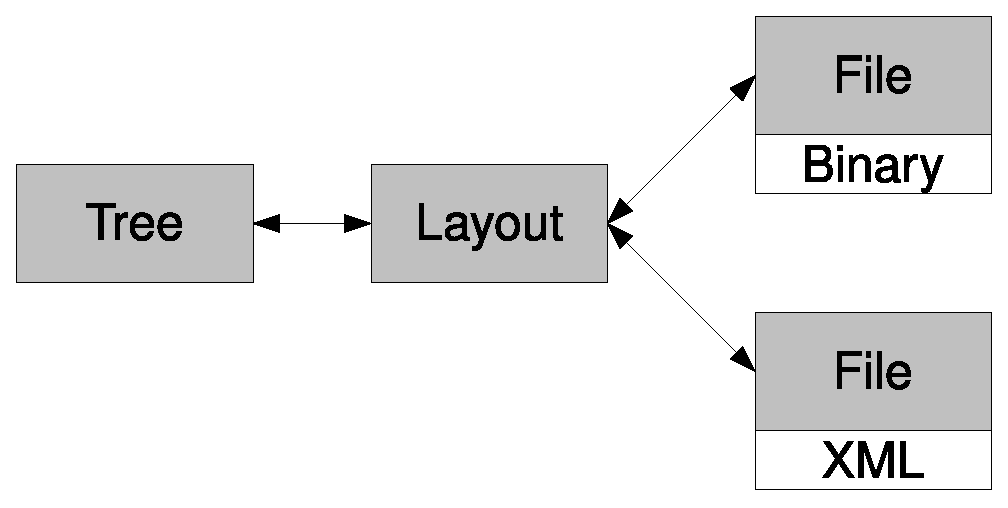
\includegraphics[scale=0.3]{guide/formats}
\caption{The four formats in which layout information can appear. The arrows mark which format can be converted in which other format. The arrows are implemented by \src{DockSituation} and \src{DockFactory}.}
\label{fig:formats}
\end{figure}

Layout information can be valid or invalid. There is only one possibility to produce invalid layout information: when reading a file in an environment that differs form the environment in which the file was written, i.e. when a \src{DockFactory} is missing. The ``tree'' must always be valid, otherwise the user would notice the errors. And \src{DockSituation} will throw an exception when attempting to write invalid layout information into a file. Hence the only format that has to support invalid layouts is the ``layout''-format.

The ''layout''-format is organized in a tree of \src{DockLayoutComposition}s. Each \src{DockLayoutComposition} represents a \src{Dockable} or a \src{DockStation} and all information that is available for them. Files on the other hand are a list of entries. Each entry contains structural information and a chunk of data. When \src{DockSituation} reads a file, it tries to map these entries to fields of \src{DockLayoutCompositions} (see figure \ref{fig:read}).

\begin{figure}[ht]
\centering
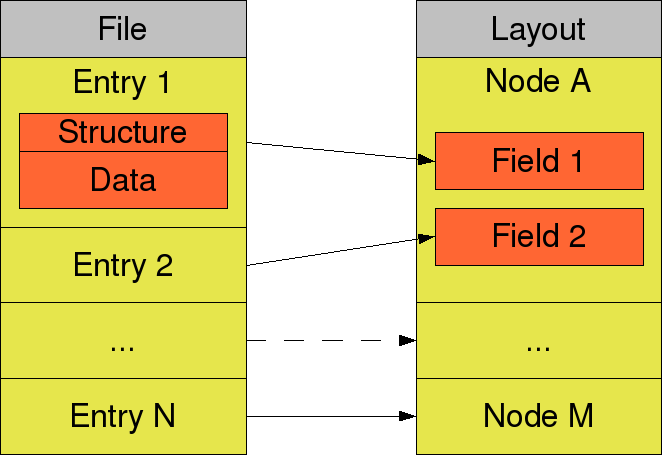
\includegraphics[scale=0.3]{guide/read}
\caption{When converting data from a file (left side) to the ``layout''-format (right side) each entry of the file is mapped to a field in one of the \src{DockLayoutComposition}s.}
\label{fig:read}
\end{figure}

A \src{DockLayoutComposition} contains three fields: \src{children}, \src{layout} and \src{adjacent}.
\begin{description}
 \item[children] If this composition represents a \src{DockStation} then this is a list of \src{DockLayoutComposition}s for the children of the station. In any other case this field is not used.
 \item[layout] This \src{DockLayoutInfo} tells how the element looks like, i.e. where to position the children. This data can either be in raw xml or binary-format, or an instance of \src{DockLayout}. In any case this data contains the unique identifier of the \src{DockFactory} which should be used to access the data.
 \item[adjacent] Additional set of data for this element. These \src{DockLayout}s are converted by \src{AdjacentDockFactory}s.
\end{description}
The data for \src{children} cannot be corrupted, however the data for \src{layout} and \src{adjacent} can. If data for \src{adjacent} is corrupted, then the entry is just ignored. If data for \src{layout} is corrupted, then the original entry in its raw format gets written into the field. While the data cannot be understood, it is still available and at its intended place. At a later point in time one might try to read that raw data again, perhaps now in an environment that understands the data.

\subsection{Local and Global: DockFrontend}
A \src{DockFrontend} uses both local and global methods to store the layout. Local methods are used when a \src{Dockable} is made visible or invisible through \src{show} and \src{hide}. Global methods are used by \src{write}, \src{read}, \src{save} and \src{load}. A \src{DockFrontend} behaves much like a \src{PredefinedDockSituation}, either elements will be created by a \src{DockFactory} or the \src{Dockables} have to be registered through \src{add}.

\section{Drag and Drop}
Drag and drop normally means grabbing a title of a \src{Dockable} by pressing the mouse, moving the mouse around, and drop the \src{Dockable} somewhere by releasing the mouse.
\subsection{Core behavior}
The sourcecode used for drag and drop operations is located in the \\\src{DockRelocator}. A \src{DockController} normally uses a \src{DefaultDockRelocator} to handle all operations. Clients seldomly need to replace the \src{DockRelocator}, but if they do, then they have to implement a new \src{DockControllerFactory} and a subclass of \src{DockController}.
\begin{lstlisting}
public class MyDockController extends DockController{
  public MyDockController(){	
    super( null );
    initiate( new DefaultDockControllerFactory(){
      @Override
      public DockRelocator createRelocator( DockController controller ) {
        return new MyDockReloactor();
      });
    }
  }
}
\end{lstlisting}
A short review of the code: the argument \src{null} line \src{3} prevents the constructor of \src{DockController} to initialize the fields. In line \src{4} the fields are initialized using a new \src{DockControllerFactory}. This factory returns a new implementation of \src{DockRelocator} in lines \src{6-8}.

\subsection{Remote control}
Sometimes the normal mechanism for drag and drop is not enough. The drag and drop operations can be called remotely using a \src{RemoteRelocator} or a \src{DirectRemoteRelocator}. Clients can request such a remote control from the \src{DockRelocator} either using \src{createRemote} or \src{createDirectRemote}.

A \src{DirectRemoteRelocator} can be used to simulate a drag and drop operation that has no real background (like a \src{MouseEvent}). A client calls \src{init} to start the operation, at least one time \src{drag} to move the grabbed \src{Dockable} around, and then \src{drop} to let the \src{Dockable} fall.

A \src{RemoteRelocator} is more tricky. The methods of a \src{RemoteRelocator} match the methods \src{mousePressed}, \src{mouseDragged} and \src{mouseReleased} of a \src{MouseListener}/\src{MouseMotionListener}. The methods \src{init}, \src{drag} and \src{drop} always tell what reaction the event caused, for example whether the operation has stopped or is going on.

\subsection{Merging}
When a \src{Dockable} is dragged over an other \src{Dockable}, then they have to be merged. The default behavior is to create a new \src{StackDockStation}, put both \src{Dockable}s onto that station, and then drop the station at the same place where the \src{Dockable}s would lie.

The creation of the station is handled by a \src{Combiner}, the \src{BasicCombiner} to be exact. Many \src{DockStation}s have a method that allows clients to set their own implementation of a \src{Combiner}. Clients can exchange the \src{Combiner} globally by creating a new \src{DockTheme}, overriding the method \src{getCombiner} and then registering a new instance at the \src{DockController} through \src{setTheme}. Note that all descendants of \src{BasicDockTheme} have a method called \src{setCombiner} that exchanges the \src{Combiner} directly without the need to override \src{getCombiner}.

\subsection{Modes}
A \src{DockRelocator} can have "modes". A mode is some kind of behavior that is activated when the user presses a certain combination of keys. Modes are modeled by the class \src{DockRelocatorMode}. It is not specified what effect a mode really has, but normally a mode would add some restrictions where to put a \src{Dockable} during drag and drop. \src{DockRelocatorMode}s can be added or removed to a \src{DockRelocator} by the methods \src{addMode} and \src{removeMode}.

Currently two modes are installed:
\begin{description}
\item[DockRelocatorMode.SCREEN\_ONLY] (press key \textit{shift}) ensures that a \\\src{Dockable} can only be put on a \src{ScreenDockStation}. That means that a \src{Dockable} can be directly above a \src{DockStation} like a \src{SplitDockStation}, but can't be dropped there.
\item[DockRelocatorMode.NO\_COMBINATION] (press key \textit{alt}) ensures that a \src{Dockable} can't be put over another \src{Dockable}. That means, every operation that would result in a merge is forbidden. Also dropping a \src{Dockable} on already merged \src{Dockable}s will not be allowed.
\end{description}

\subsection{Restrictions}
Sometimes a developer wishes to restrict the set of possible targets for a drop-operation. There are multiple reasons why someone would like to do that:
\begin{itemize}
 \item Some \src{Dockable} must always be visible
 \item Some \src{DockStation}s represent a special area that can only be used by some \src{Dockable}s
 \item Some \src{Dockable}s can only be presented on a certain kind of \src{DockStation}
\end{itemize}

There are also a lot of ways how to achieve this goal.
\begin{itemize}
 \item Every \src{Dockable} has two methods called \src{accept}. One of them tells the system, whether a \src{Dockable} accepts some \src{DockStation} as parent or not. The other tells whether the \src{Dockable} can be merged with another \src{Dockable}.
 \item Each \src{DockStation} has a method \src{accept}. This method tells whether some \src{Dockable} can become a child of the \src{DockStation}.
 \item And then there are \src{DockAcceptance}s. A \src{DockAcceptance} has \src{accept}-methods too. These methods get a \src{DockStation} and some \src{Dockable}s, and then have to decide whether the elements can be put together. Each \src{DockAcceptance} works on a global scale, and thus they are registered at the \src{DockController} through \src{addAcceptance}.
\end{itemize}

\section{Themes}
A \src{DockTheme} is nothing else than a \src{LookAndFeel} for DockingFrames. Each \src{DockController} can have exactly one \src{DockTheme} at any given time. The \src{DockTheme} contains a set of icons, painting code, behaviors and other stuff, that changes the way a user interacts with DF.

\begin{lstlisting}
DockController controller = ...
DockTheme theme = new EclipseTheme();
controller.setTheme( theme );
\end{lstlisting}
The previous listing shows how easy it is to set the theme. All that needs to be done is to create the desired theme (line \src{2}) and set it (line \src{3}).

Several \src{DockTheme}s are already part of DF. An easy way to access all of them is the method \src{getThemes} of \src{DockUI}. This method returns a set of \src{ThemeFactory}s which then can create some \src{DockTheme}s.

\subsection{Themes of DF}
This section lists all \src{DockTheme}s that are in DF and mentions their specialities, if there are any.
\subsubsection{BasicTheme}
The \src{BasicTheme} is a very simple implementation. Its strength is, that it shows as much features as possible. If there is the possibility to show some button, then some button is shown. If there is the possibility to add a border to a \src{Component}, then a border is added. While \src{BasicTheme} does not look very nice to the user, it does make debugging a lot easier.
\subsubsection{SmoothTheme}
\src{SmoothTheme} is almost the same as \src{BasicTheme}, but the titles that are shown for each \src{Dockable} have been replaced. They have now a smooth animation that is triggered whenever the focused \src{Dockable} changes.
\subsubsection{FlatTheme}
The reverse of \src{BasicTheme}, this theme does not add any borders, buttons or other decorations unless necessary. It's not a very complex theme, and easy to understand by a user.
\subsubsection{BubbleTheme}
A more experimental theme. It uses animations and graphical gimmicks wherever possible. This theme has some issues with performance, but it is certainly a good demonstration of the potential of the theming-mechanism.
\subsubsection{EclipseTheme} \label{EclipseTheme}
The \src{EclipseTheme} tries to imitate the behavior of the famous Eclipse platform. It changes the behavior of DF massivly. Some properties of \src{EclipseTheme} can be set through the \src{DockProperties} as in the following example.
\begin{lstlisting}
DockController controller = ...
DockProperties properties = controller.getProperties();
properties.set(
	EclipseTheme.PAINT_ICONS_WHEN_DESELECTED,
	true );
\end{lstlisting}
Let's have quick look: in line \src{1} we get some \src{DockController}. In line \src{2} we get access to the set of properties. In line \src{3-5} the property \\\src{PAINT_ICONS_WHEN_DESELECTED} is set to \src{true}.

There are more properties for \src{EclipseTheme}:
\begin{description}
 \item[TAB\_PAINTER] tells how to paint tabs on the \src{StockDockStation}. Possible values are \src{ShapedGradientPainter.FACTORY}, \\\src{RectGradientPainter.FACTORY}, \src{DockTitleTab.FACTORY} or any other \\\src{TabPainter}.
 \item[THEME\_CONNECTOR] tells which kind of title and border should be used for \src{Dockable}s, and which actions should be displayed on the tabs (actions on the tabs are always visible, other actions are only visible when a \src{Dockable} is selected). The value can be any \src{EclipseThemeConnector}.
 \end{description}

A note: if no special theme-connector is used, then any action that is marked with the annotation \src{EclipseTabDockAction} will be shown on the tabs.

\subsubsection{NoStackTheme}
This \src{DockTheme} takes another theme and changes its behavior. In particular it removes some titles and ensures, that no \src{StackDockStation}s are put in another. That ensures that merged \src{Dockable}s are not merged again. A behavior that a user might like better then the original behavior, because it is harder to loose a \src{Dockable}.

The use of \src{NoStackTheme} is simple:
\begin{lstlisting}
DockController controller = ...
DockTheme theme = ...
conroller.setTheme( new NoStackTheme( theme ));
\end{lstlisting}

\subsection{How to write your own DockTheme}
Writing a \src{DockTheme} is a complex matter. If you'd like to write a theme then you should make some preparations:
\begin{enumerate}
 \item Write at least one application using DF
 \item Read this document, twice
 \item Download the source of DF, download the API-documentation
 \item Have a look how other themes are made, \src{FlatTheme} is a good mix of simplicity and small features. You can learn a lot just analyzing \src{FlatTheme}
 \item Look up any unknown interface in the API-documentation or in the source
\end{enumerate}

The best way to start is by creating a subclass of \src{BasicTheme}. \src{BasicTheme} will ensure that you have someting that works and that you can modifie step by step. As you will see, \src{BasicTheme} has many \src{setXYZ}-methods, refer to step 5 of your preparations and look at the API-documentation to find out, what these methods do.

There is method called \src{install}. This method can be overriden (don't forget to call \src{super.install}) and changes any property of a \src{DockController}. The most often used objects by \src{install} are:
\begin{description}
 \item[IconManager] contains all \src{Icon}s that are used, the \src{Icon}s can be exchanged.
 \item[DockTitleManager] contains factories which will create the titles for some \src{Dockable}s.
 \item[ActionViewConverter] contains factories which create views for actions (for example a \src{JButton} for a \src{ButtonDockAction})
 \item[DockProperties] is a map for all sorts of properties, can be used as cheap distribution system for values that must be known globally
\end{description}

Don't forget to undo the changes in the method \src{uninstall}.

\subsection{UI properties}
There are resources that need to be distributed through the whole user interface, for example colors. An easy way is just to have some map with \src{String}-resource pairs. The \src{UIProperties} is just such a map with a few extras.

Components that use \src{UIProperties} do not just ask for a resource when they need it, they register an \src{UIValue} which gets informed whenever the resource changes. At a first glance \src{UIValue} is just an observer of the map.

The map does not forward its resources directly to the \src{UIValue}s, it forwards the resources and the values to an \src{UIBridge}. The bridge is then responsible to forward the resource to its \src{UIValue}. Each kind of \src{UIValue} can have its own bridge (the kind is defined through a \src{Path} object). The \src{UIBridge} can modify the resource before sending it to the \src{UIValue}. If a subclass of \src{UIValue} would have a \src{Dockable} field, then a bridge for that subclass could make its decision based on the value of that field.

\src{UIBridges} are also informed about which \src{UIValue}s are observing the \\\src{UIProperties}. A bridge could decide to change the resource of a \src{UIValue} when the \src{UIProperties} did not change at all. The \src{UIValue} would not be able to tell the difference.

There is currently one \src{UIProperties} used in the core for colors and another one for fonts.

\subsection{Colors}
Since DF is a graphical user interface, colors are used often and by a all sorts of components. The most important colors are collected in a map, and components get their colors from that color-map.

There is no repository for the keys of the color-map, nor any rule how to choose them. But each class that uses the color-map, should have the annotation \src{ColorCodes}. All keys should be listed as arguments. The annotation is for documentation only.

Components do not ask the color-map directly for a color, they register a \src{DockColor}-object at the map. \src{DockColor} is just an observer which gets informed whenever a color in the map changes. That allows to exchange colors while the components are visible, and the changes are immediately visible.

There are different subclasses of \src{DockColor}. Each subclass tells by whom the color is used, for example a \src{TitleColor} would be used by a specific \src{DockTitle}.

Clients can exchange and influence the colors on different levels.

\subsubsection{ColorScheme}
The \src{BasicTheme} uses a \src{ColorScheme} to put up its set of colors. \src{ColorScheme} has one important method: \src{getColor}. That method gets a key for a color, and has to return the color that matches. The \src{ColorScheme} of \src{BasicTheme} can be replaced at any time calling the method \src{setColorScheme} or through the \src{DockProperties} using the key \src{BasicTheme.BASIC_COLOR_SCHEME}. Note that subclasses might use another key for the \src{ColorScheme}. Since all \src{DockTheme}s of the core library inherit \src{BasicTheme}, the possibility to use a \src{ColorScheme} is available for all themes.

\subsubsection{ColorManager}
Instead of putting all colors at once, using a \src{ColorScheme}, a single color can be set with the \src{ColorManager}. The \src{ColorManager} is accessible through the method \src{DockController.getColors}. Clients can just call the method \src{put} to put a new color into the color-map. The \src{ColorManager} is an \src{UIProperties} and hence has the ability to use \src{UIBridge}s. The \src{ColorManager} requires to use the subinterface \src{ColorBridge} instead of \src{UIBridge}.

\section{Actions}
A \src{DockAction} is an object which is related to one or many \src{Dockable}s, they describe some action like "close a \src{Dockable}". Every \src{DockAction} has the ability to create one or many views of itself. A view might be a \src{JButton}, a \src{JCheckBox}, a \src{JMenuItem} or other objects.

Every \src{Dockable} has a list of associated \src{DockAction}s. This list is modeled by a \src{DockActionSource}. 

If some module wants to show the actions of a \src{Dockable}, it asks for the \src{Dockable}s global \src{DockActionSource}, then it commands each \src{DockAction} to create a view that can be displayed by the module. A \src{JMenu} will ask for another type of view than a \src{DockTitle} would. So the menu might get a \src{JMenuItem}, the title a \src{JButton}.

Let's write a simple action.
\begin{lstlisting}
public class CloseAction extends SimpleButtonAction{
	public CloseAction(){
		setText( "Close" );
		setTooltip( "Removes this panel from the view" );
		setIcon( new ImageIcon( "close.png" ));
		setAccelerator(
			 KeyStroke.getKeyStroke(
				KeyEvent.VK_C,
				KeyEvent.CTRL_DOWN_MASK ) );
	}

	@Override
	public void action( Dockable dockable ){
		super.action( dockable );
		DockStation parent = dockable.getDockParent();
		if( parent != null )
			parent.drag( dockable );
	}
}
\end{lstlisting}
One of the predefined \src{DockAction}s is used to implement the new kind of action. The \src{SimpleButtonAction} is an action that behaves like a push-down-button. In lines \src{3-9} some properties are set that help the user to understand and access \src{CloseAction}. The logic of the action is written down in lines \src{14-17}. In this case, a \src{Dockable} is removed from its parent.

And now lets add \src{CloseAction} to the list of actions some \src{Dockable} offers. Since \src{DefaultDockable} will be the most often used implementation of \src{Dockable}, the example uses a \src{DefaultDockable} as well.
\begin{lstlisting}
DefaultDockable dockable = ...
CloseAction action = new CloseAction();

DefaultDockActionSource source = new DefaultDockActionSource(
	new LocationHint(
		LocationHint.DOCKABLE, 
		LocationHint.RIGHT_OF_ALL ));
source.add( action );
dockable.setActionOffers( source );
\end{lstlisting}
In line \src{4} a new \src{DockActionSource} is created. The \src{LocationHint} in lines \src{5-7} tells everyone, that the origin of \src{source} is a \src{Dockable}, and that \src{source} should be on the right side if the content of many \src{DockActionSource}s are displayed in a row. The new \src{CloseAction} is inserted into \src{source} at line \src{8}. Then the list of actions of \src{dockable}s is changed to \src{source} in line \src{9}. Note that lines \src{8} and \src{9} could be exchanged without any effect to the rest of the program.

\subsection{Sources of DockActions}
So how exactly does a module find out, which \src{DockAction}s to show for a \src{Dockable}? The module uses the method \src{Dockable.getGlobalActionOffers} to optain a \src{DockActionSource}. The result of \src{getGlobalActionOffers} is a composite of \src{DockActionSource}s. The children of the result come from different sources:
\begin{description}
 \item[Local DockActionSource] Every \src{Dockable} should have a local list of actions, this list can be accessed through \src{getLocalActionOffers}. Some implementations of \src{Dockable} have a method that allows clients to exchange that local list. For example \src{setActionOffers} in \src{DefaultDockable}.
 \item[Through the parents] Most \src{Dockable}s have one or more \src{DockStation}s as parents. Each \src{DockStation} can offer \src{direct} (if direct parent) or \\\src{indirect} (if grandparent) \src{DockActionSource}s for each child. Clients rarely interfere in that mechanism.
 \item[Guards] \src{ActionGuard}s observe all \src{Dockable}s of a \src{DockController}. They can react to a \src{Dockable} and add additional \src{DockActionSource}s. An \src{ActionGuard} has to be made registered by calling \src{addActionGuard} of \\\src{DockController}.
 \item[Alternative sources] The \src{ActionOffer} normally is the authority that creates the content of the global \src{DockActionSource}. A \src{Dockable} will get one \src{ActionOffer} and give that offer all \src{DockActionSource}s that were gathered. Then the \src{ActionOffer} will determine in which order the \\\src{DockActionSource}s appear and create a new composite of the sources. Clients can add new \src{ActionOffer}s by calling \src{addActionOffer} of \\\src{DockController}.
 \end{description}

\subsection{Kinds of DockActions}
There are different kinds of \src{DockAction}, all with different behavior. 

There is a list of concepts that describe the most often used kinds of actions:
\begin{description}
 \item[Button-DockAction] This kind of action reacts like a button. They can be triggered over and over again, always calling the same piece of code.
 \item[CheckBox-DockAction] This kind has two states: selected and not-selected. Every time the action is triggered, the state changes.
 \item[RadioButton-DockAction] Like the \src{CheckBox}-kind, but many \\\src{RadioButton}s are grouped together, and only one of them can be selected. Triggering a not-selected button will deselect the currently selected button.
 \item[Menu-DockAction] These actions just open some pop-up menu that contains another set of actions.
 \item[DropDown-DockAction] Like the \src{Menu}-kind, but this action also remembers which child was triggered earlier. This last triggered child can be called again without the need to open the pop-up menu.
\end{description}

All these concepts are implemented by the "simple" \src{DockAction}s:
\begin{center}
% use packages: array
\begin{tabular}{ll}
\textbf{Kind} & \textbf{Action} \\
Button & \src{SimpleButtonAction} \\
CheckBox & \src{SimpleSelectableAction.Check} \\ 
RadioButton & \src{SimpleSelectableAction.Radio} \\ 
Menu & \src{SimpleMenuAction} \\
DropDown & \src{SimpleDropDownAction}
\end{tabular}
\end{center}

There is also a more complex series of actions, called the "grouped" \\\src{DockAction}s. The grouped actions do not store single properties like the simple actions, they store maps of properties. Each \src{Dockable} that is bound to a grouped action is then associated with one key, and that key is used to read the maps.

As an example: a grouped action that counts for each \src{Dockable} how many times the action was triggered. When testing this action you will note that certain events (like changing the \src{DockTheme}) set the counter back to 0. It is never safe to store information in a grouped action.
\begin{lstlisting}
public class CountingAction extends GroupedButtonDockAction<Integer>{
	public CountingAction() {
		super( null );
		setGenerator( new GroupKeyGenerator<Integer>(){
			public Integer generateKey( Dockable dockable ) {
				return 0;
			}
		});
		setRemoveEmptyGroups( true );
	}

	@Override
	protected SimpleButtonAction createGroup( Integer key ) {
		SimpleButtonAction group = super.createGroup( key );
		group.setText( String.valueOf( key ) );
		return group;
	}

	public void action( Dockable dockable ) {
		String text = getText( dockable );
		int count = Integer.valueOf( text );
		count++;
		setGroup( count, dockable );
	}
}
\end{lstlisting}
In lines \src{4-8} a \src{GroupKeyGenerator} is set. This generator will determine the initial group of each new \src{Dockable}. In line \src{9} the fate of empty groups is defined. Empty groups are to be deleted. That is a good behavior if groups are generated automatically and the number of groups is unknown. The code in lines \src{13-17} defines how a new group is created. And finally in lines \src{20-23} the count-event is handled. The action will be triggered for \src{dockable}, and putting \src{dockable} in a new group changes the text on each view that shows the action for \src{dockable}.

There are a few grouped actions defined in DF:
\begin{center}
% use packages: array
\begin{tabular}{ll}
\textbf{Kind} & \textbf{Action} \\
Button & \src{GroupedButtonDockAction} \\
CheckBox & \src{GroupedSelectableDockAction.Check} \\ 
RadioButton & \src{GroupedSelectableDockAction.Radio} \\ 
Menu & - \\
DropDown & -
\end{tabular}
\end{center}

Finally there is a very small action called \src{SeparatorAction}. This action just adds a line or space in the view, acting as a separator between other actions.

\subsection{Lifecycle}
Eventually each \src{DockAction} is instantiated and stored at a place where it can be found. While a \src{DockAction} enters and leaves the realm of a \src{DockController}, these things might happen.
\begin{enumerate}
 \item Every time some module is going to use an action, it connects the \\\src{DockAction} with one or many \src{Dockable}s (the method \src{bind} is called). This call informs the \src{DockAction} that it is related to the \src{Dockable}s.
 \item A module normally wants to show some view for an action. Therefore it calls \src{DockAction.createView}. It gives \src{createView} a \src{ViewTarget}. A \src{ViewTarget} tells what kind of view is requested, one for a menu, one for a title or even something that is defined by the client. The module also gives an \src{ActionViewConverter} to \src{createView}. The \src{ActionViewConverter} is a set of factories which can create the views that are often needed. Most \src{DockAction}s will tell the converter what type of action they are (with an argument of type \src{ActionType}) and what \src{ViewTarget} the module requests. Then the converter will create a view matching the parameters.
 \item Most views have some binding mechanism that has to be used by the module. This binding mechanism will install or uninstall some listeners when needed.
 \item When a module no longer uses an action, it disconnects the \src{DockAction} from one or many \src{Dockable}s (the method \src{unbind} is called). That informs the \src{DockAction} to remove all ties to these \src{Dockable}s, releasing as many resources as possible.
\end{enumerate}
Clients might be interested to introduce new kinds of views or new types of actions.
\begin{itemize}
 \item When a client adds a new kind of view, it has to define a new \\\src{ViewTarget}. The client then has to register a new \src{ViewGenerator} for each type of action at the \src{ActionViewConverter}.
 \item When a client adds a new type of action, it has to define a new \\\src{ActionType}. The client then has to register a new \src{ViewGenerator} for each kind of view at the \src{ActionViewConverter}.
\end{itemize}

Let's have a look at an example. In the example a new kind of view and a new kind of action will be introduced.
\begin{lstlisting}
    ViewTarget<JButton> TOOLBAR = 
        new ViewTarget<JButton>( "toolbar" );
    
    ActionType<TextAction> TEXT_ACTION =
        new ActionType<TextAction>( "text_action" );
\end{lstlisting}
First the new kind of view \src{TOOLBAR} and the new type of action \src{TEXT_ACTION} is defined. Lines \src{1,2} say that the view will only consist of \src{JButton}s. Lines \src{4,5} define that the new type of action is always a \src{TextAction}. So the next step is to define \src{TextAction}.
\begin{lstlisting}
    public class TextAction implements DockAction{
        public void bind( Dockable dockable ) {
            // ignore
        }
        
        public String getContent(){
            return "text";
        }

        public <V> V createView( ViewTarget<V> target, 
                ActionViewConverter converter, Dockable dockable ) {
            
            return converter.createView( TEXT_ACTION, this, target, dockable ); 
        }

        public boolean trigger( Dockable dockable ) {
            // ignore
            return false;
        }

        public void unbind( Dockable dockable ) {
            // ignore
        }    
    }
\end{lstlisting}
As can be seen in line \src{1}, \src{TextAction} is an implemtation of \src{DockAction}. Since this action is rather stupid, we can ignore most input. Line \src{13} is the most important line, here an \src{ActionViewConverter} is used to create a view for the \src{TextAction}. Note that the action has to pass \src{TEXT_ACTION}, the type of action it is.

Since the \src{ActionViewConverter} does not know \src{TOOLBAR} or \src{TEXT_ACTION}, a \src{ViewGenerator} has to be defined. In fact there are several \src{ViewGenerator}s necessary, one for each combination of \src{ViewTarget} and \src{ActionType}. But in this example only one new generator is written.
\begin{lstlisting}
public class ToolbarTextAction implements ViewGenerator<TextAction, JButton>{
	public JButton create(
		ActionViewConverter converter,
		final TextAction action,
		final Dockable dockable ) {

		String content = action.getContent();
		JButton button = new JButton( content );
		button.addActionListener( new ActionListener(){
			public void actionPerformed( ActionEvent e ) {
				action.trigger( dockable );
			}
		});
		return button;
	}
}
\end{lstlisting}
Note how the generator can make use of the knowledge, that it receives a \src{TextAction}. In line \src{7} it asks for the content of the action, a method only available for \src{TextAction}s. The generator also connects view and action, in this case by adding a \src{ActionListener} to \src{button}.

Finally the new generator has to be made public:
\begin{lstlisting}
DockController controller = ...
ActionViewConverter converter = controller.getActionViewConverter();

converter.putDefault( 
	TEXT_ACTION,
	TOOLBAR,
	new ToolbarTextAction() );
\end{lstlisting}
There are several methods called \src{putX} in \src{ActionViewConverter}. \src{putDefault} should be used for new generators, \src{putTheme} is only used by \src{DockTheme}s, and \src{putClient} can be used by any client to override values that were set by \src{putDefault} or \src{putTheme}.

A module that needs a view for \src{TOOLBAR} would later call code that looks like this:
\begin{lstlisting}
ActionViewConverter converter = ...
TextAction action = ...
Dockable dockable = ...

JButton button = converter.createView( action, TOOLBAR, dockable )
\end{lstlisting}

\section{Titles}
A \src{DockTitle} is a \src{Component} that shows the icon, title-text, actions and/or other information related to a \src{Dockable}. A drag and drop operation is most often initiated by the mouse grabbing a \src{DockTitle}.

\subsection{New titles}
There is not much help to offer for developers which want to write a new kind of title. However there are some classes which might help:
\begin{description}
 \item[AbstractDockTitle] offers all the features a \src{DockTitle} should have, subclasses can override \src{paintBackground} to add their own painting code.
 \item[BasicDockTitle] paints some gradient as background. Clients can change these colors.
 \item[ButtonPanel] a \src{Component} that can display a set of \src{DockAction}s. Clients just invoke \src{set(Dockable)} to show the actions of a particular \src{Dockable}. If there is not enough space for all \src{DockAction}s, then \src{ButtonPanel} can use an additional pop-up for the abundant actions.
\end{description}

\subsection{Lifecycle}
If a module wants to show a \src{DockTitle} for a \src{Dockable}, what has it to do? First a module needs to define what kind of \src{DockTitle} it wants to show. For that it needs the \src{DockTitleManager} which is available through a \src{DockController}. The module then calls \src{getVersion(String,DockTitleFactory)} to optain a \src{DockTitleVersion}. A \src{DockTitleVersion} describes the kind of a \src{DockTitle}.

Later when the module gets a \src{Dockable}, it invokes \src{Dockable.getDockTitle} with its \src{DockTitleVersion}. A \src{Dockable} can decide on its own how to create the title, but most \src{Dockable}s will simply call \src{DockTitleVersion.createDockable}.

If the module got a title (and not \src{null}), it binds the title to its \src{Dockable} calling \src{Dockable.bind(DockTitle)}. The \src{DockController} will handle any other binding operations that need to be done.

When a module no longer needs a \src{DockTitle}, it unbinds the title through \src{Dockable.unbind(DockTitle)}.

Clients can influence the \src{DockTitle} that is used for a \src{Dockable} in two ways:
\begin{itemize}
 \item They override \src{Dockable.getDockTitle} and return any title they like.
 \item They install a new \src{DockTitleFactory} at the \src{DockTitleManager}. Clients can do this by invoking \src{registerClient(String,DockTitleFactory)}.
\end{itemize}

\section{Preferences}
The preference system was introduced with version 1.0.6 of the core library.

If a setting is meaningful for the ordinary user, and the user would like to be able to change the setting, then this setting should be made accessible through a preference. For example the shortcut to maximize a \src{Dockable} (ctrl+m) is a good candidate for a preference.

So what is a preference? A preference is a representation of some kind of property in a unified way. It is a mediator between the system in which the property is stored, and the graphical user interface and storage mechanisms written for preferences.

Each preference consists of some properties:
\begin{description}
 \item[Value] The thing which the user would like to change.
 \item[ValueInfo] Information about the value, for example the maximum value for an \src{Integer}-value. The exact meaning of this property depends on the \src{TypePath}.
 \item[TypePath] The type tells how to work with the value, how to present it to the user or how to write it as xml. The type is represented by a \src{Path}-object. It is a \src{Path} and not a \src{Class} object because many preference-types may use the same objects as value. For example an unbounded \src{Integer} versus an \src{Integer} which must be in the range 1 to 10.
 \item[Path] A unique path to this preference. Used as an identifier if preferences have to be stored in some kind of map.
\end{description}

\subsection{Organization}
The basic module of the preference system is the \src{PreferenceModel}. 

Most methods of the \src{PreferenceModel} are simple to understand and do not need a discussion. Those which are part of a greater scheme however will receive some attention in this chapter.

In the preference system a \src{PreferenceModel} is just a layer above some kind of storage mechanism for the real properties. It is most often used as a mediator and a buffer between that storage mechanism and the algorithms that want to use the preferences (for example a user interface). The methods \src{read} and \src{write} are used to access the covered storage mechanism. The method \src{read} will read values from the storage mechanism into the model. The method \src{write} will write the values back into that storage mechanism.

\subsection{Models}
There are some implementations of \src{PreferenceModel} already in the core library.

\subsubsection{DefaultPreferenceModel}
This model uses a list of \src{Preference}-objects to represent the preferences. All the properties needed for a preference are stored in such a \src{Preference}-object. The API-documentation reveals that there are many \src{Preference}s representing different aspects of the core library. For example there is a \src{Preference} which represents the keystroke for maximizing a \src{Dockable}.

There are also subclasses of \src{DefaultPreferenceModel}. These subclasses are collections of preferences which belong together, for example the \\\src{EclipseThemePreferenceModel} which contains preferences that are related to the \src{EclipseTheme}.

\subsubsection{MergedPreferenceModel}
This model is a list of other models. It just takes the preferences from these other models and presents them as its own preferences. It offers a quick and simple way to create a combination of two ore more models.

\subsubsection{PreferenceTreeModel}
This model is a \src{PreferenceModel} and a \src{javax.swing.TreeModel}. If seen as \src{PreferenceModel}, then it behaves like a \src{MergedPreferenceModel}. If seen as \src{TreeModel}, then it contains \src{PrefereceTreeModel.Node}-objects. A node can either be just a name, or another \src{PreferenceModel}. This model is intended to be used in a \src{JTree} where the user can select one aspect of the whole set of preferences to show.

The subclass \src{DockingFramesPreferenceModel} is the set of preferences \\which includes all the aspects of the core-library.

\subsection{Lifecycle}
This section describes the best way how to use a \src{PreferenceModel}. Not everything used in this section is explained yet, so you might want to read this section a second time when you finished this whole chapter.

The correct lifecycle of a \src{PreferenceModel} includes normally these steps:
\begin{enumerate}
 \item Create the model. Set up all the preferences that are used by the model.
 \item Call \src{load} on a \src{StoragePreference}.
 \item Call \src{write} on the model to synchronize the model with the underlying system.
 \item (work with the underlying system)
 \item To work with the model: call first \src{read}, then make the changes in the model, then call \src{write}.
 \item (work with the underlying system)
 \item Call \src{read} on the model to synchronize the model with the underlying system.
 \item Store the model using \src{store} of a \src{PreferenceStorage}.
\end{enumerate}

If the \src{PreferenceStorage} used in step \src{2} is empty because its \src{read} or \src{readXML} method failed, then calling \src{read} of \src{PreferenceModel} would at least load some default settings.

Steps \src{4, 5, 6} can be cycled as many times as needed.

An additional step \src{0} and \src{9} would be to read and write the \\\src{PreferenceStorage} when starting up or shuting down the application.

\subsection{User Interface}
If a \src{PreferenceModel} should be displayed, the \src{PreferenceTable} can be used. This table shows a label and an editor for each preference. For \\\src{PreferenceTreeModel}s a \src{PreferenceTreePanel} should be used, it shows a \\\src{PreferenceTable} and a \src{JTree} for the nodes of the \src{PreferenceTreeModel}.

Clients can also use a \src{PreferenceDialog} or a \src{PreferenceTreeDialog} to show a dialog with the well known buttons "ok" and "cancel".

\subsubsection{Editors}
Since there are different types of preferences, different editors are needed. The kind of editor for one preference is determined by the type-path (\src{getTypePath} in a model). Clients can add new editors to a \src{PreferenceTable} through the method \src{setEditorFactory}.

An editor is always of type \src{PreferenceEditor}. Each editor gets a \\\src{PreferenceEditorCallback} with which it can interact with the table. Whenever the user changes the editors value, the editor should call the method \src{set} of \src{PreferenceEditorCallback} to make sure the new value gets stored.

\subsubsection{Operators}
There are some operations which should be available for almost any preference. For example \textit{set a default value} or \textit{delete the current value}. The preference system introduces the \src{PreferenceOperation} to handle this kind of actions.

A \src{PreferenceOperation} is nothing more than a label and an icon. The logic for an operation is either in an editor or in a model.

\begin{description}
 \item[Editor:] Editors with operations must call the method \src{setOperation} of \\\src{PreferenceEditorCallback} for each operation they offer. By calling \src{setOperation} more than once, the editor can change the enabled state of the operation. If the user triggers an operation of the editor, the method \src{doOperation} of \src{PreferenceEditor} is called. It is then the editors responsibility to handle the operation.
 \item[Preference:] Preferences can have operations as well. The method \\\src{getOperations} of \src{PreferenceModel} will be called once to get all the available operations for one preference. The method \src{isEnabled} will be invoked to find out whether an operation is enabled or not. Models can change the enabled state by calling \src{preferenceChanged} of \\\src{PreferenceModelListener}. If the user triggers an operation, \\\src{doOperation} of \src{PreferenceModel} will be invoked.
\end{description}
If an editor and a preference share the same operations, then per definition the operations belong to the editor. All settings from the model will just be ignored.

\subsection{Storage}
The \src{PreferenceStorage} can be used to store \src{PreferenceModel}s in memory or persistent either as byte-stream or as XML.

The normal way to write a model from memory to the disk looks like this:
\begin{lstlisting}
// the stream we want to write into
DataOutputStream out = ...

// the model we want to store
PreferenceModel model = ...

// And now store the model
PreferenceStorage storage = new PreferenceStorage();
storage.store( model );
storage.write( out );
\end{lstlisting}
Note that there are two phases in writing \src{model}. First the model gets \src{store}d (line \src{9}) into \src{storage}. It is possible to store more than just one model in a \src{PreferenceStorage}. Second \src{storage} gets written onto the disk in line \src{10}.

The standard way to read a model are to apply the same steps in reverse:
\begin{lstlisting}
// the source of any new data
DataInputStream in = ...

// the model we want to load
PreferenceModel model = ...

// And now load the model
PreferenceStorage storage = new PreferenceStorage();
storage.read( in );
storage.load( model, false );
\end{lstlisting}
Like writing this operation has two phases. In line \src{9} \src{storage} gets filled with information, in line \src{10} the information gets transfered to \src{model}. The argument \src{false} is a hint what to do with missing preferences. In this case missing preferences are just ignored. A value of \src{true} would force them to become \src{null}.

There are some preferences which do not need to be stored by the \\\src{PreferenceStorage} because they are already stored by the underlying systen. These preferences are called \textit{natural}, while the others are called \textit{artificial}. The method \src{isNatural} of \src{PreferenceModel} can be used to distinguish them.


\section{Global Properties}
Every \src{DockController} has map that contains global properties. There are no restrictions to what a property can be, a \src{Boolean} could be a property of a \src{KeyStroke}. 

Clients may use the map for their own purposes.

The map itself is an instance of \src{DockProperties} and can be accessed with the method \src{DockController.getProperties}. The keys for the map are of type \\\src{PropertyKey}. Each key needs a generic argument, that ensures that there are no casting problems.

Clients can add a \src{DockPropertyListener} to the map. This listener will be informed whenever the property of a specified key changes.

Clients might also use a \src{PropertyValue}, which is a \src{DockPropertyListener} that can attach itself to a \src{DockProperties}. A \src{PropertyValue} has also the ability to override the value it normaly reads from the map by a custom value.

This chapter will now list up all keys and their meanings that are present in DF. 

\begin{itemize}
\item \src{PropertyKey.DOCKABLE_ICON} An \src{Icon} that is shown in the title of a \src{Dockable} if the \src{Dockable} has no \src{Icon} of its own.
\item \src{PropertyKey.DOCKABLE_TITLE} A \src{String} that is shown as text in the title of a \src{Dockable} if the \src{Dockable} has no title text of its own.
\item \src{PropertyKey.DOCK_STATION_ICON} A \src{Icon} that is shown in the title of a \src{DockStation} if the \src{DockStation} does not have an \src{Icon} of its own.
\item \src{PropertyKey.DOCK_STATION_TITLE} A \src{String} that is shown as text in the title of a \src{DockStation} if the \src{DockStation} does not have a title text of its own.
\item \src{EclipseTheme.PAINT_ICONS_WHEN_DESELECTED} A \src{Boolean} that tells \\whether \src{Icon}s are painted on tabs if the tabs are not selected. Please refer to the chapter \ref{EclipseTheme}.
\item \src{EclipseTheme.TAB_PAINTER} A \src{TabPainter} used by the \src{EclipseTheme} to paint the tabs. Please refer to the chapter \ref{EclipseTheme}.
\item \src{EclipseTheme.THEME_CONNECTOR} An \src{EclipseThemeConnector} that tells the \src{EclipseTheme} how put up its layout. Please refer to the chapter \ref{EclipseTheme}.
\item \src{DockableSelector.INIT_SELECTION} A \src{KeyStroke} that activates the \\\src{DockableSelector}. The selector then allows the user to select a \src{Dockable} which gains the focus. The default value is set to \src{ctrl + shift + e}.
\item \src{DockRelocatorMode.NO_COMBINATION_MASK} A \src{ModifierMask} that tells which keys have to be pressed in order to activate the no-combination-mode when dragging around a \src{Dockable}. The default value is set to \src{alt}.
\item \src{DockRelocatorMode.SCREEN_MASK} A \src{ModifierMask} that tells which keys have to be pressed in order to activate the drop-on-screen-only-mode when dragging around a \src{Dockable}. The default value is set to \src{shift}.
\item \src{FlapDockStation.BUTTON_CONTENT} A value of the enumeration \\\src{ButtonContent}. Tells the \src{FlapDockStation} how to paint the buttons of its children. The default is set to \src{THEME_DEPENDENT} which leaves the choice to the current \src{DockTheme}.
\item \src{FlapDockStation.LAYOUT_MANAGER} The \src{FlapLayoutManager} that is used by all \src{FlapDockStation}s. That layout manager can store the \src{hold}- and the \src{size}-property of children of \src{FlapDockStation}. The default value is an instance of \src{DefaultFlapLayoutManager} which does not store anything.
\item \src{ScreenDockStation.BOUNDARY_RESTRICTION} A \src{BoundaryRestriction} \\that will be used by \src{ScreenDockStation} to determine where to put its dialogs. The interface \src{BoundaryRestriction} contains already some constant restrictions: \src{FREE} that allows anything (and is the default value), and \src{HARD} which is very restrictive.
\item \src{SplitDockStation.LAYOUT_MANAGER} The \src{SplitLayoutManager} that will be used by \src{SplitDockStation} to validate its content and to perform drag and drop operations. This value normaly is an instance of \\\src{DefaultSplitLayoutMangaer}. 
\item \src{SplitDockStation.MAXIMIZE_ACCELERATOR} A \src{KeyStroke} that changes the maximized-state of \src{SplitDockStation} assuming that a \\\src{SplitDockStation} or one of its children has the focus. The default is set to \src{ctrl + m}.
\item \src{StackDockStation.COMPONENT_FACTORY} This key represents a \\\src{StackDockComponentFactory} that is used by the \src{StackDockStation} to create its content. A warning: this key is used by many \src{DockTheme}s to exchange the look of \\\src{StackDockStation}.
\item \src{DockFrontend.HIDE_ACCELERATOR} The \src{KeyStroke} that is used to activate the hide-action (also known as close-action) when using a \src{DockFrontend}. The default value for this key is \src{ctrl + F4}
\item \src{BasicTheme.BASIC_COLOR_SCHEME} \\\src{BubbleTheme.BUBBLE_COLOR_SCHEME} \\\src{EclipseTheme.ECLIPSE_COLOR_SCHEME} \\\src{FlatTheme.FLAT_COLOR_SCHEME}: The \src{ColorScheme} used for various \\\src{DochTheme}s.
\item \src{AWTComponentCaptureStrategy.STRATEGY} How to create a picture of a \src{java.awt.Component} which is not from the Swing package.
\end{itemize}

\end{document}







